\section{Asset Allocation with Transaction Costs}

\begin{frame}{Problem Formulation}
	\onslide<1->{
	\begin{block}{Investor's Goal}
		How to dynamically invest the available capital in a portfolio of different assets in order to maximize the expected total return or another relevant performance measure.
	\end{block}
	}
	
	\onslide<2->{
	\textbf{Rewards}: portfolio log-return with transaction costs
		\begin{equation*}
			R_{t+1} = \log \left\{ 1 + \sum^{I}_{i=0} \left[ 
				\tikz[baseline]{
		        	\node[anchor=base] (t1) {$a_t^i X_{t+1}^i$};
		        } - 
		        \tikz[baseline]{
		        	\node[anchor=base] (t2) {$\delta_i \left| a_t^i - \widetilde{a}_t^i \right|$};
		       	} -
		       	\tikz[baseline]{
		       		\node[anchor=base] (t3) {$\delta_s {(a_t^i)}^-$};
		       	} \right] -
		       	\tikz[baseline]{
		       		\node[anchor=base] (t4) {$\delta_f \mathbf{1}_{{a}_t \neq \tilde{{a}}_{t-1}}$};
		       	} \right\}	 	
		 \end{equation*}
	}
	
	\onslide<7->{
	\textbf{Actions}: Portfolio weights
		\begin{equation*}
			\{a_t^i\}_{i=0}^I \;\;\; \text{s.t.}\;\;\; \sum^{I}_{i=0} a_t^i = 1 \;\;\;\;\; \forall t \in \{0, 1, 2, \ldots\}
		\end{equation*}
	}

	\onslide<8->{
	\textbf{States}: assets past returns and current allocation
		\begin{equation*}
			S_t = \{X, X_t, X_{t-1}, \ldots, X_{t-P}, \tilde{a}_t\}
		\end{equation*}
	}
	
	\onslide<3|handout:0>{
		\begin{tikzpicture}[overlay]
				\node[draw=SteelBlue, circle, line width=3pt, minimum size=2cm] at (t1) {};
		\end{tikzpicture}
	}
	
	\onslide<4|handout:0>{
		\begin{tikzpicture}[overlay]
				\node[draw=SteelBlue, circle, line width=3pt, minimum size=2cm] at (t2) {};
		\end{tikzpicture}
	}
		
	\onslide<5|handout:0>{
		\begin{tikzpicture}[overlay]
				\node[draw=SteelBlue, circle, line width=3pt, minimum size=2cm] at (t3) {};
		\end{tikzpicture}
	}
			
	\onslide<6|handout:0>{
		\begin{tikzpicture}[overlay]
				\node[draw=SteelBlue, circle, line width=3pt, minimum size=2cm] at (t4) (g) {};
		\end{tikzpicture}
	}
\end{frame}

\begin{frame}[c]{Synthetic Asset: Convergence}
\begin{figure}[t!]
	\centering
	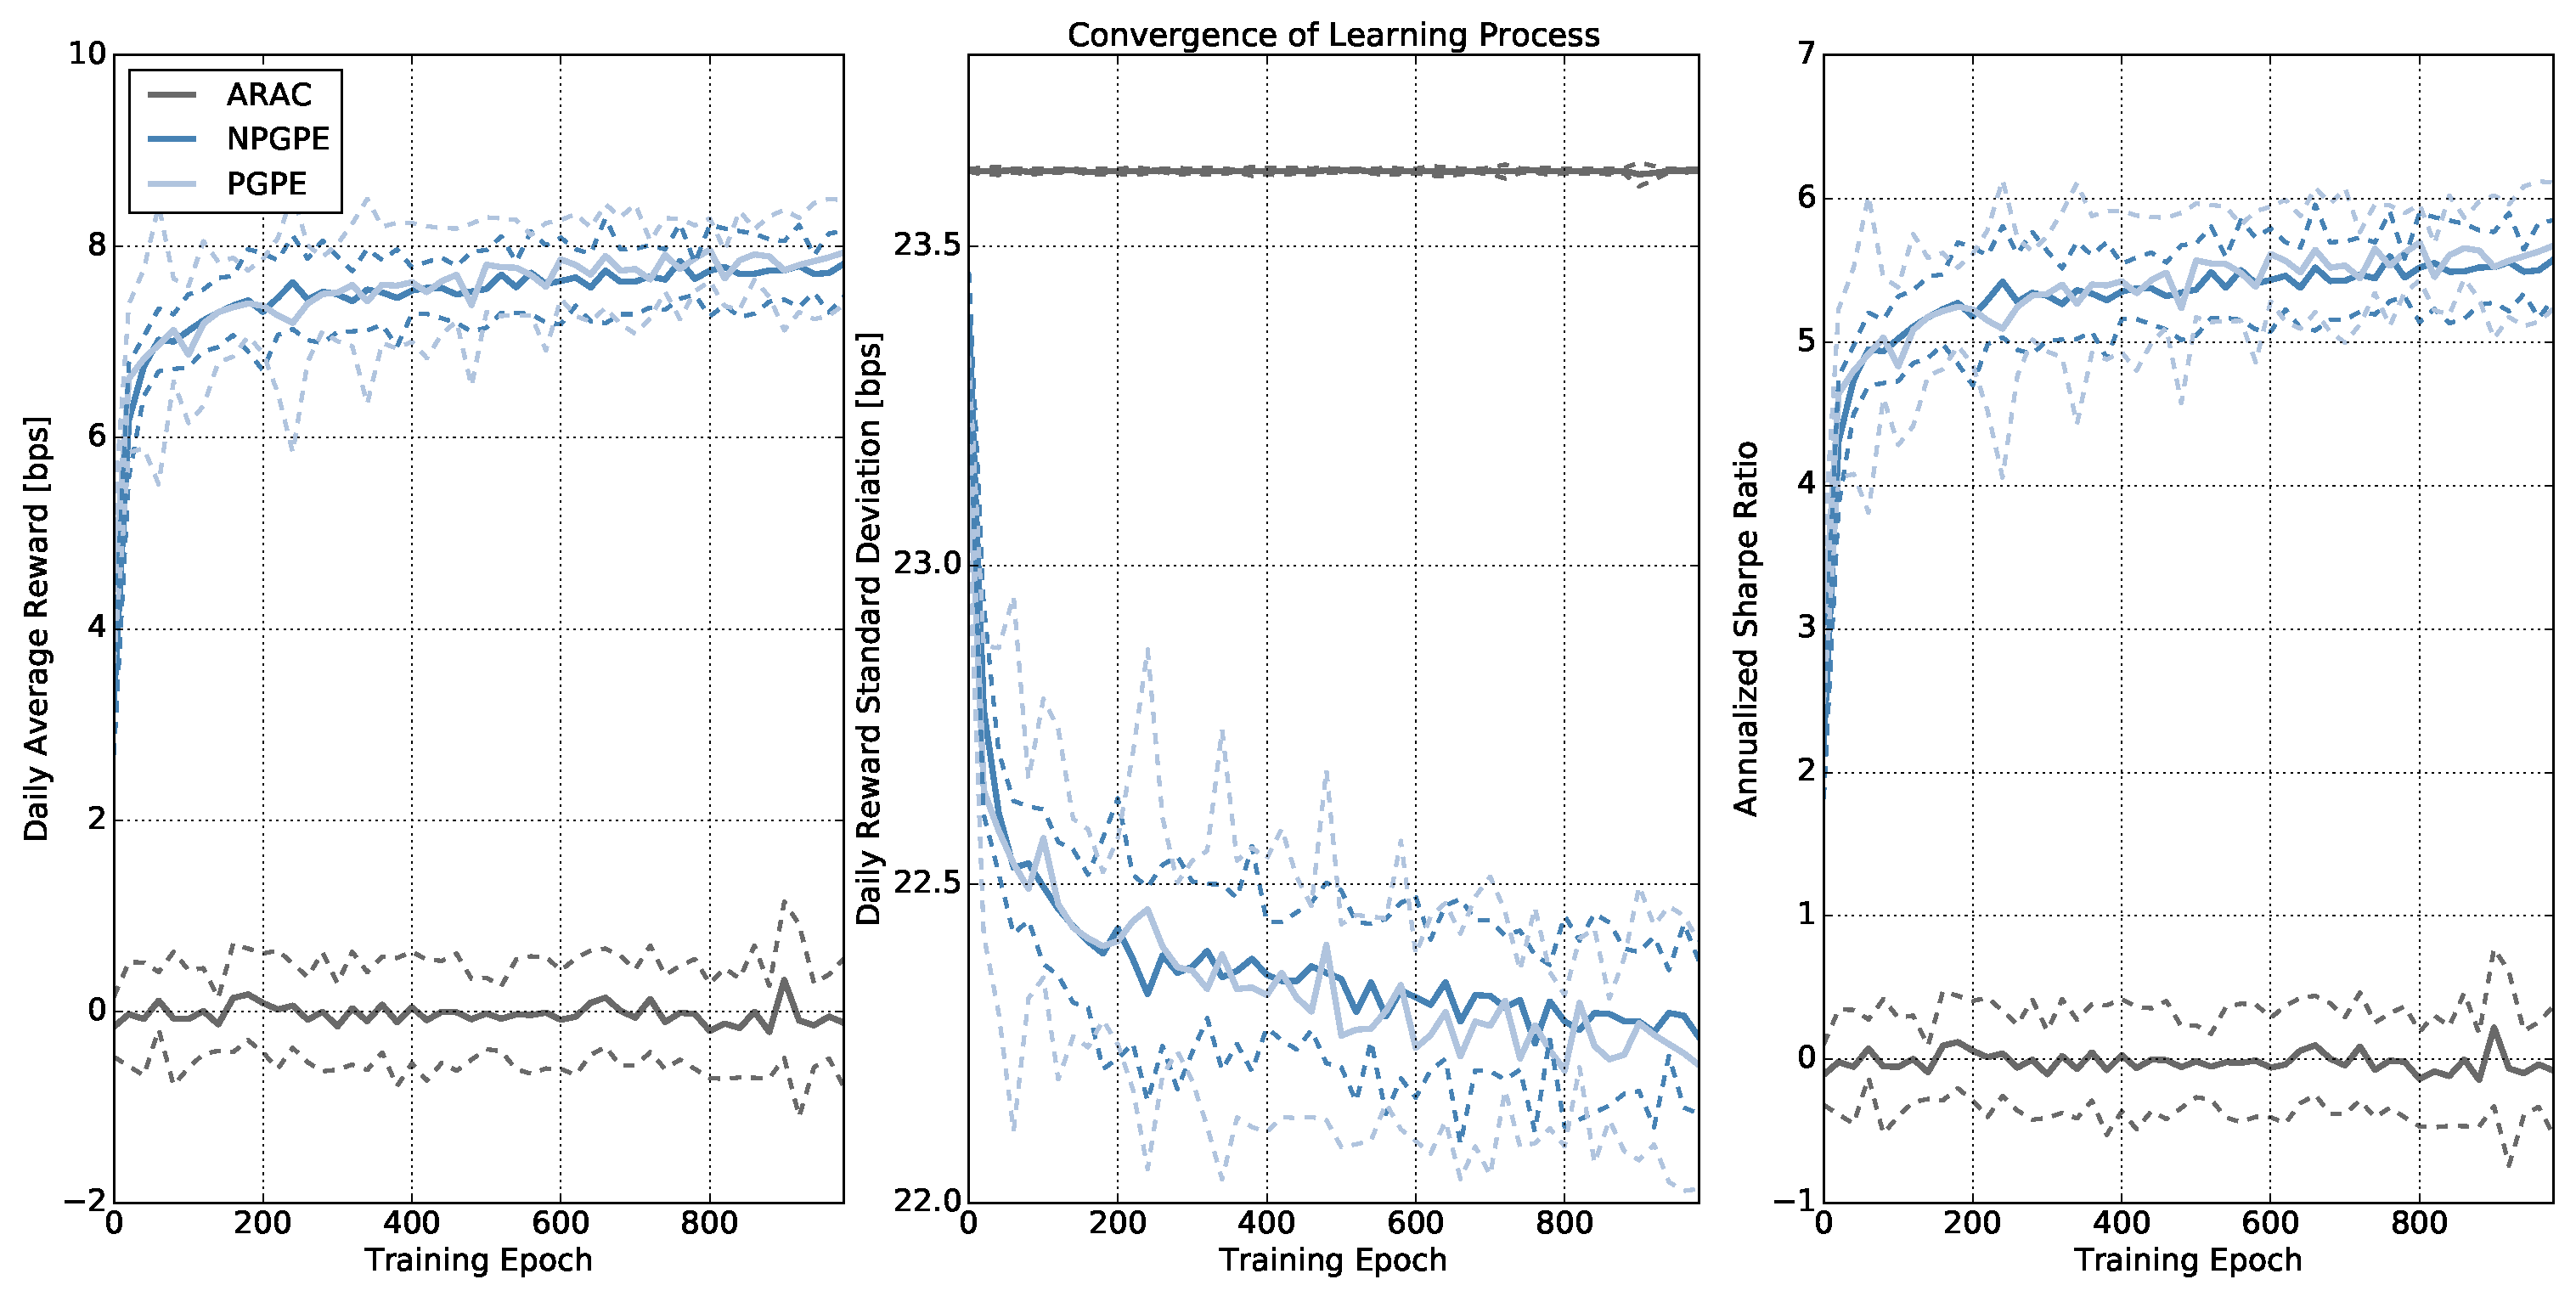
\includegraphics[height=5cm,width=0.8\textwidth]{Images/6_0_single_synthetic_neutral_convergence}
\end{figure}
\end{frame}


\begin{frame}[c]{Synthetic Asset: Backtest Performance}
\begin{figure}[t]
	\centering
	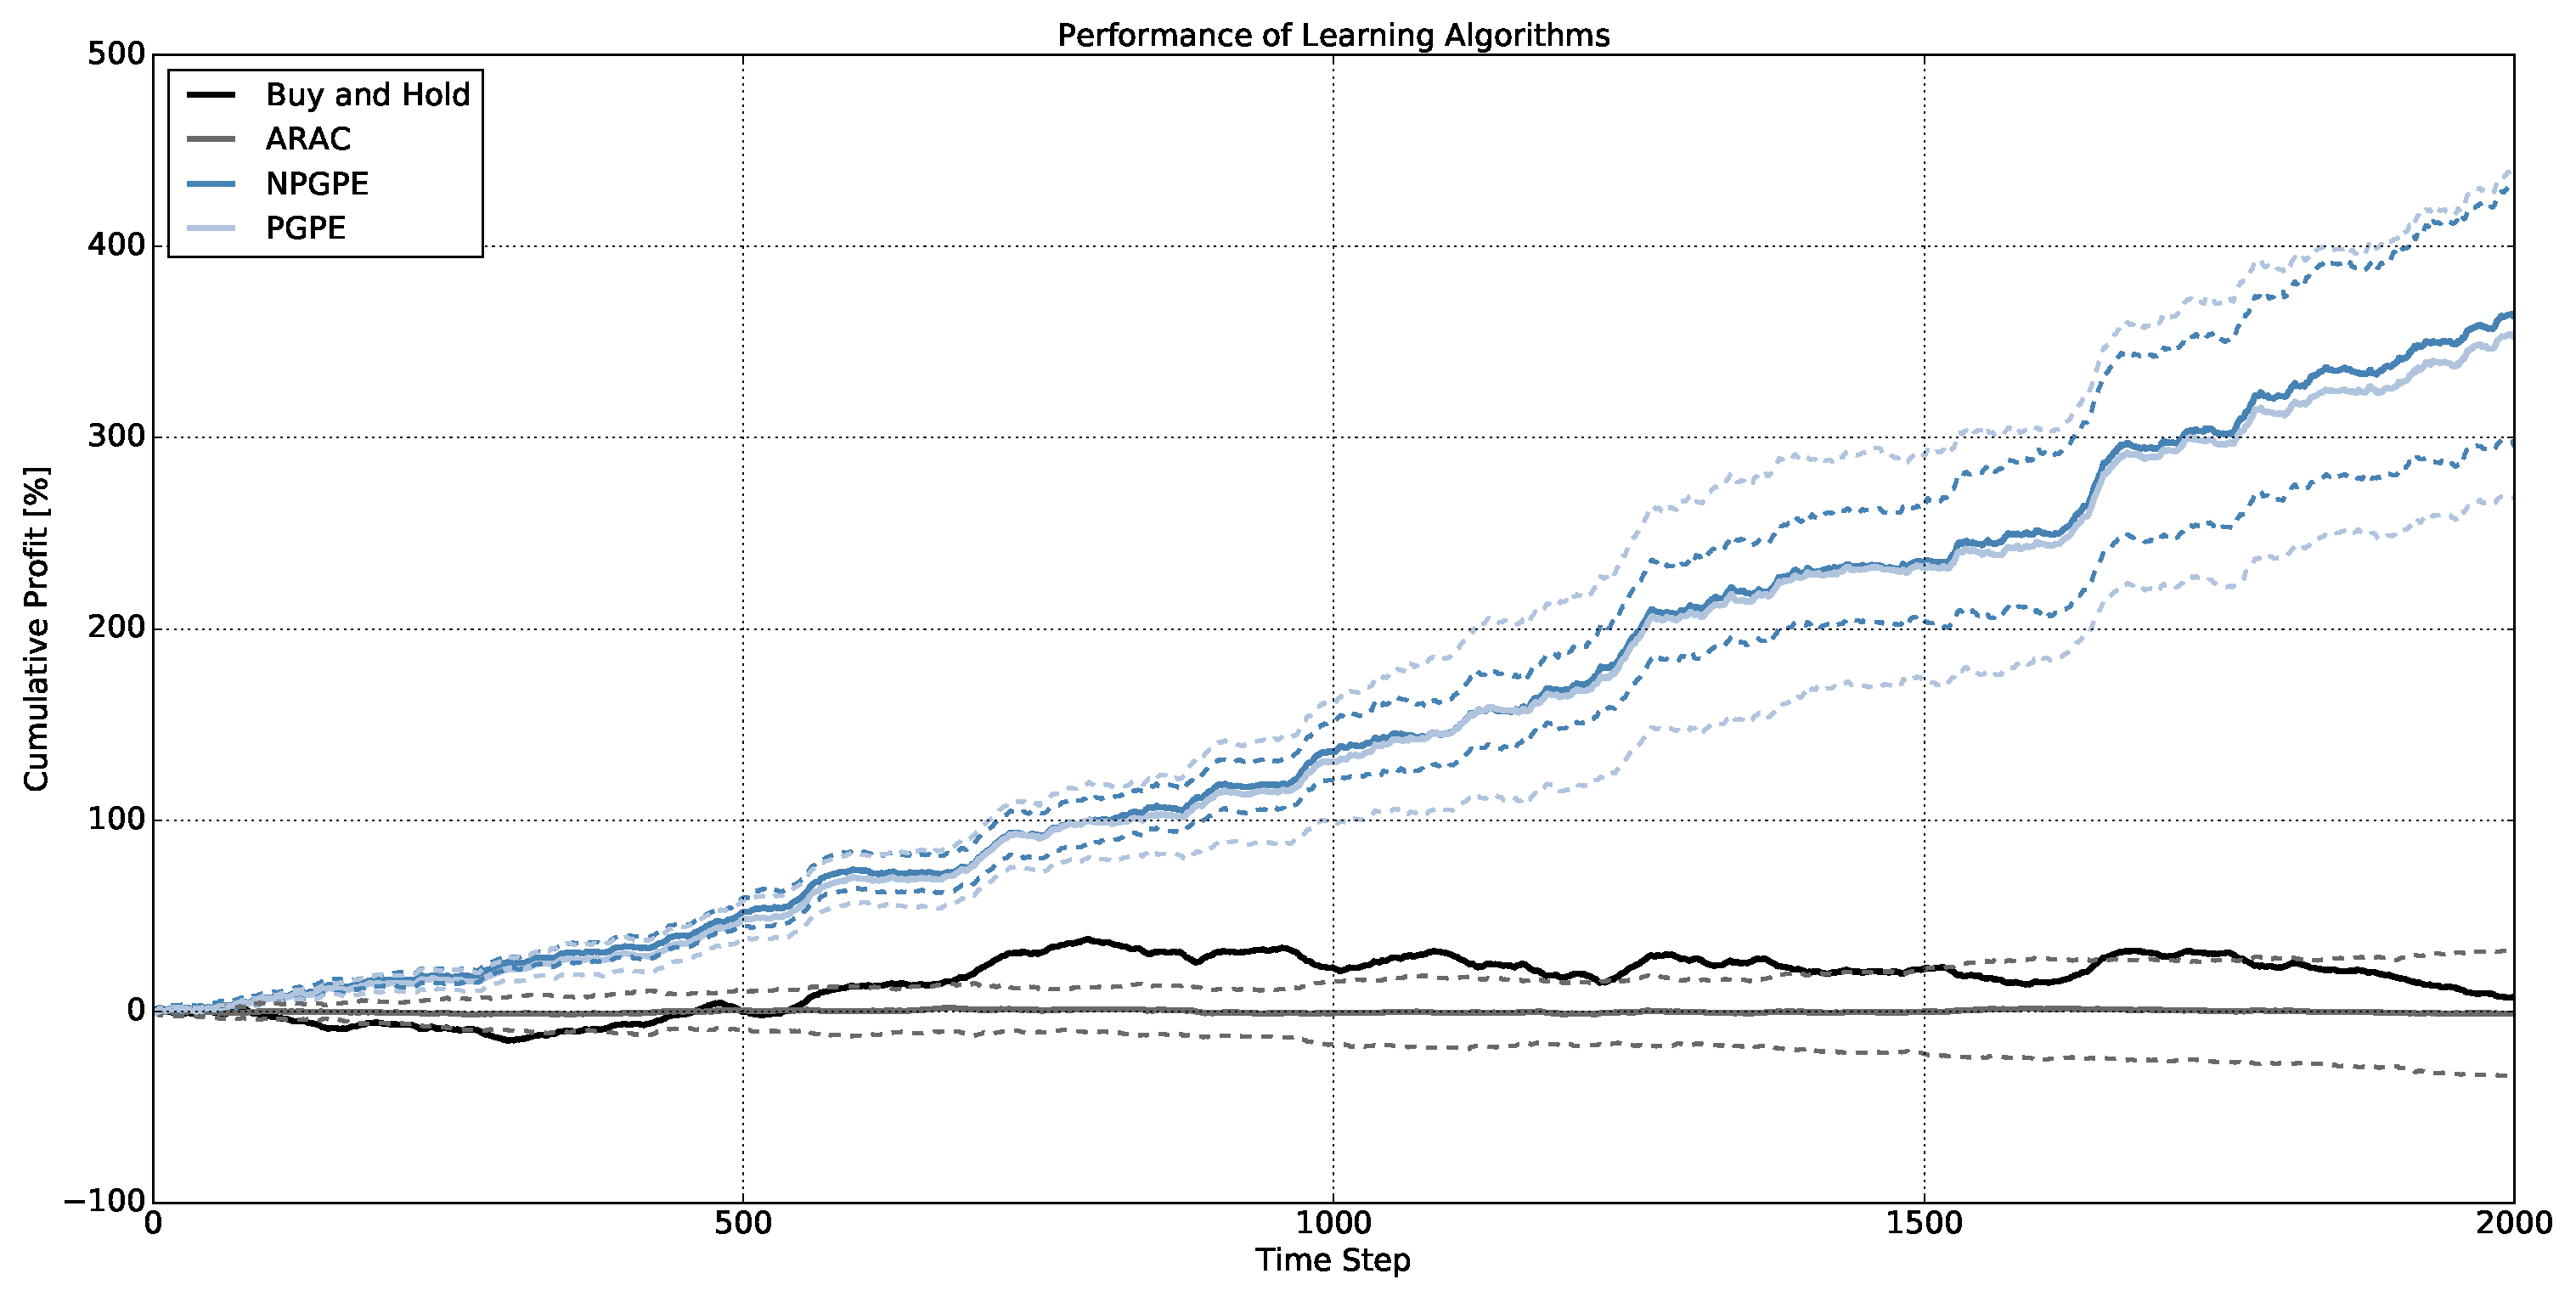
\includegraphics[height=6cm,width=0.8\textwidth]{Images/6_1_single_synthetic_neutral_performance}
\end{figure}
\end{frame}

\begin{frame}[c]{Synthetic Asset: Impact of Transaction Costs}
\begin{figure}[t!]
	\centering
	\includegraphics[height=3cm,width=0.8\textwidth]{Images/6_2_impact_transaction_costs}
\end{figure}
\begin{figure}[t!]
	\centering
	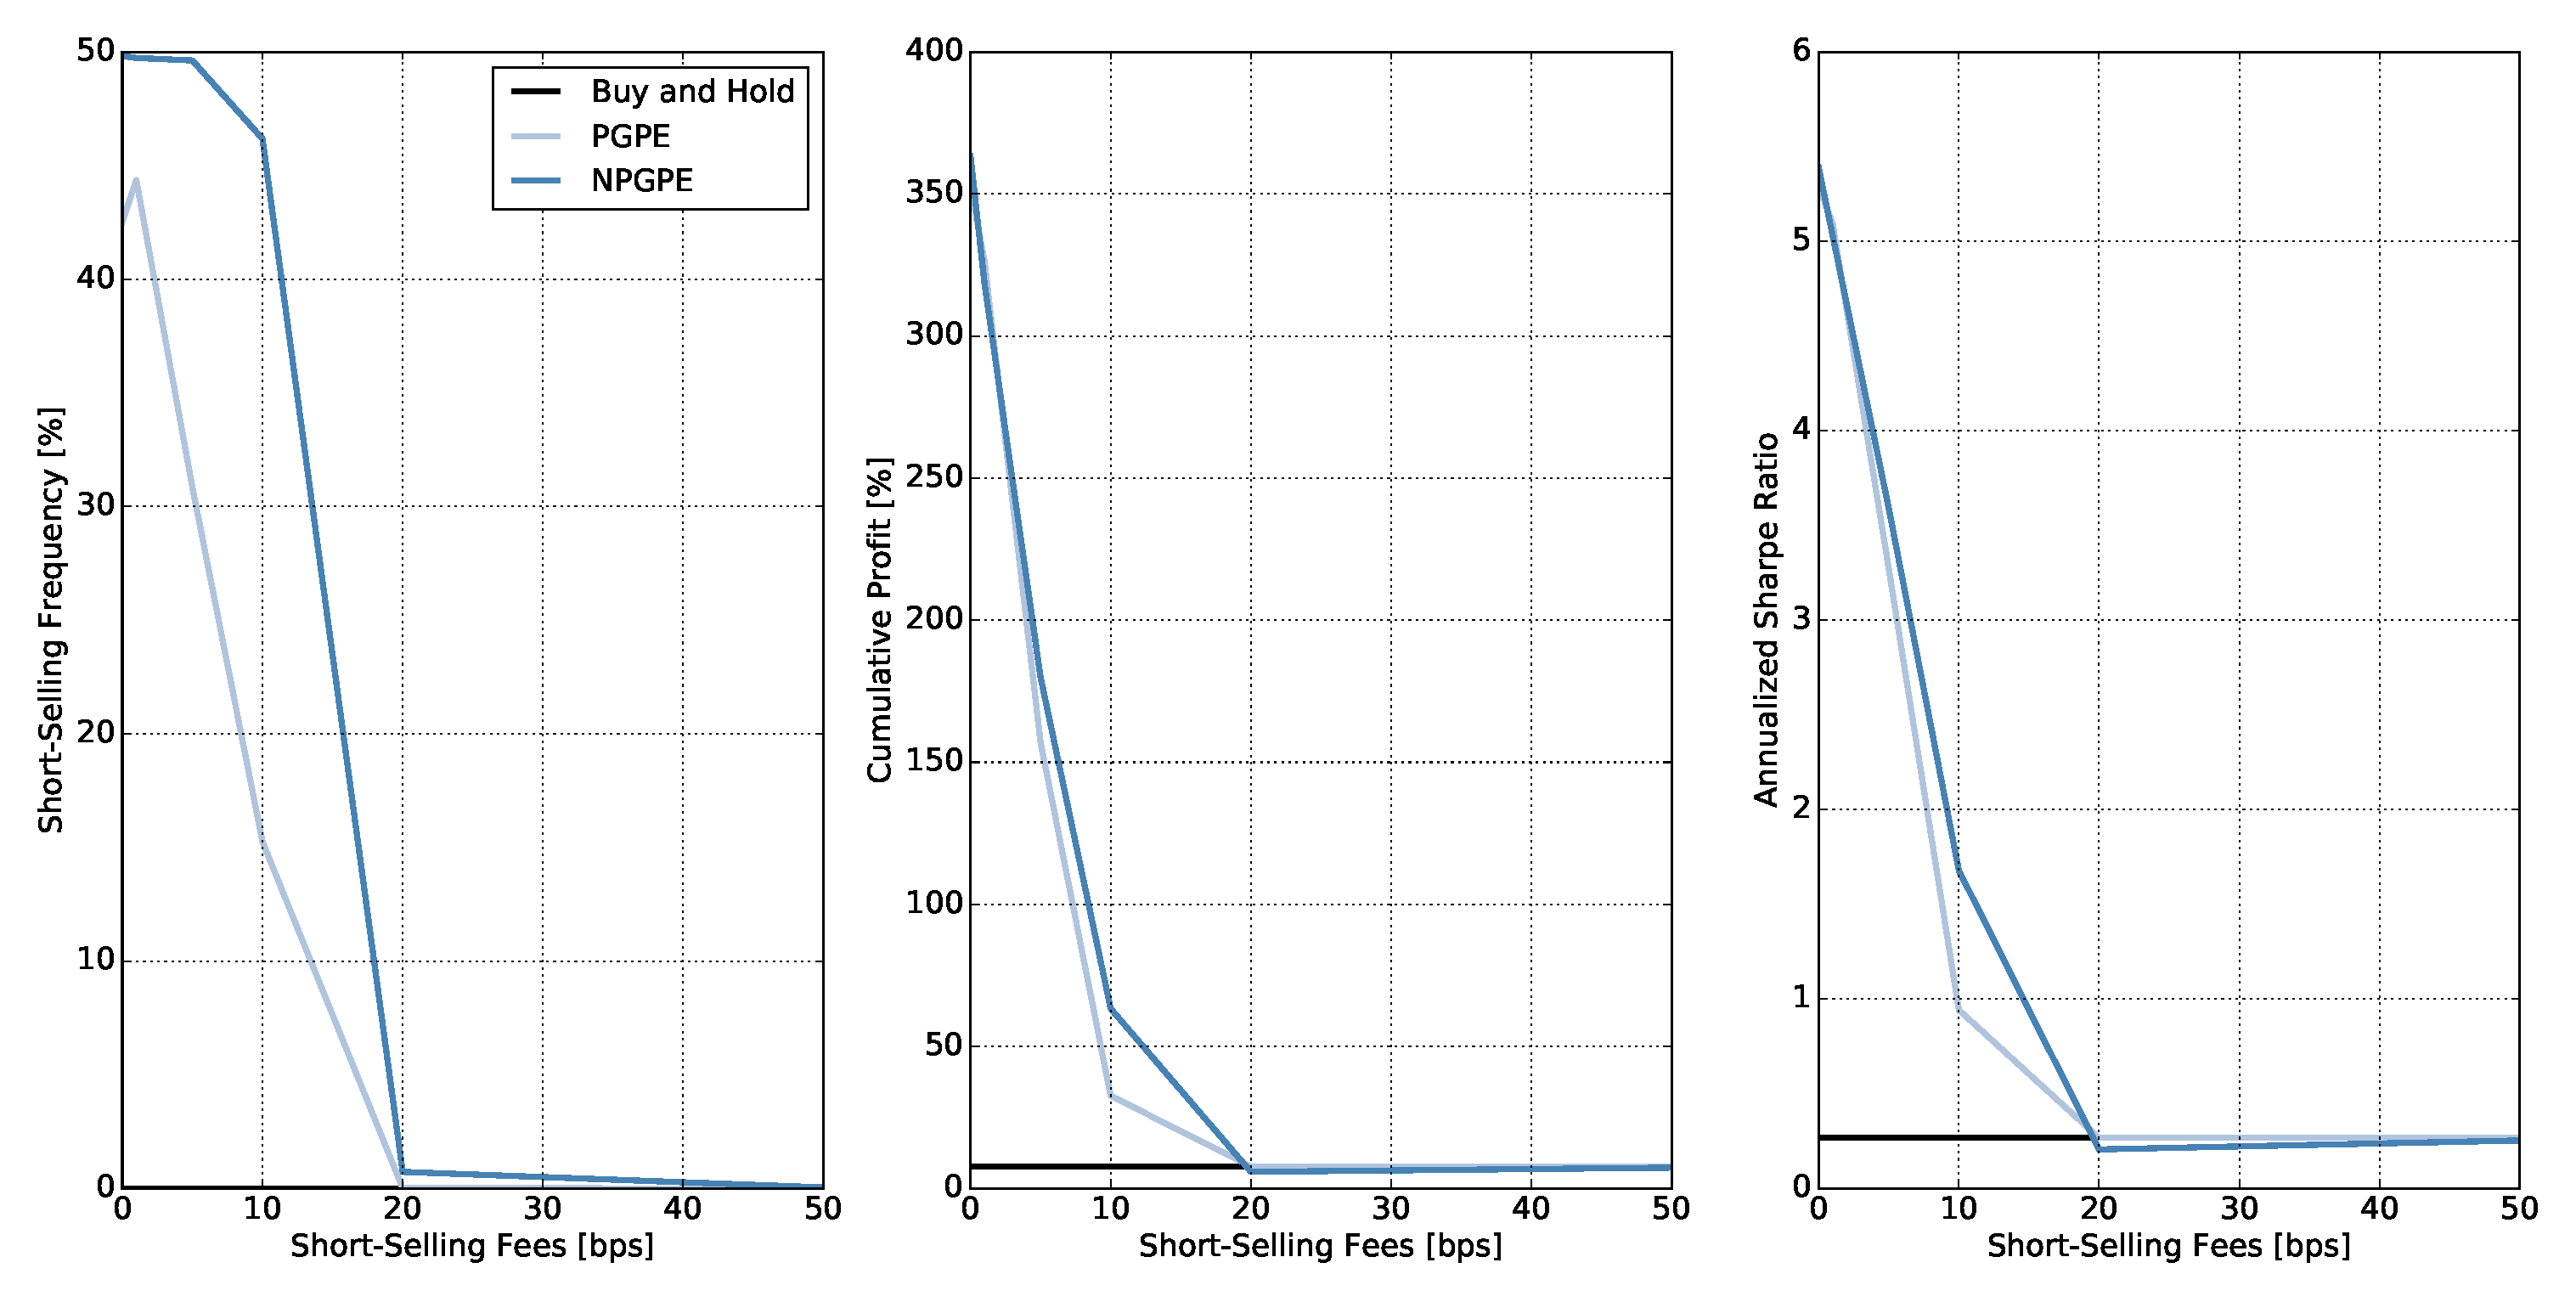
\includegraphics[height=3cm,width=0.8\textwidth]{Images/6_3_impact_short_selling_fees}
\end{figure}
\end{frame}

\begin{frame}{Not So Fast}

	\onslide<1->{
	\begin{columns}
	\begin{column}{0.6\textwidth}
	   \begin{alertblock}{Insuccess on Historical Data}
	   Successfully applying these RL algorithms to historical data is much more challenging
	   \begin{enumerate}
	   		\item Fail to converge
	   		\item The strategies learned are not profitable
	   \end{enumerate}
	   \end{alertblock}
	\end{column}
	\begin{column}{0.4\textwidth}
	    \begin{center}
	     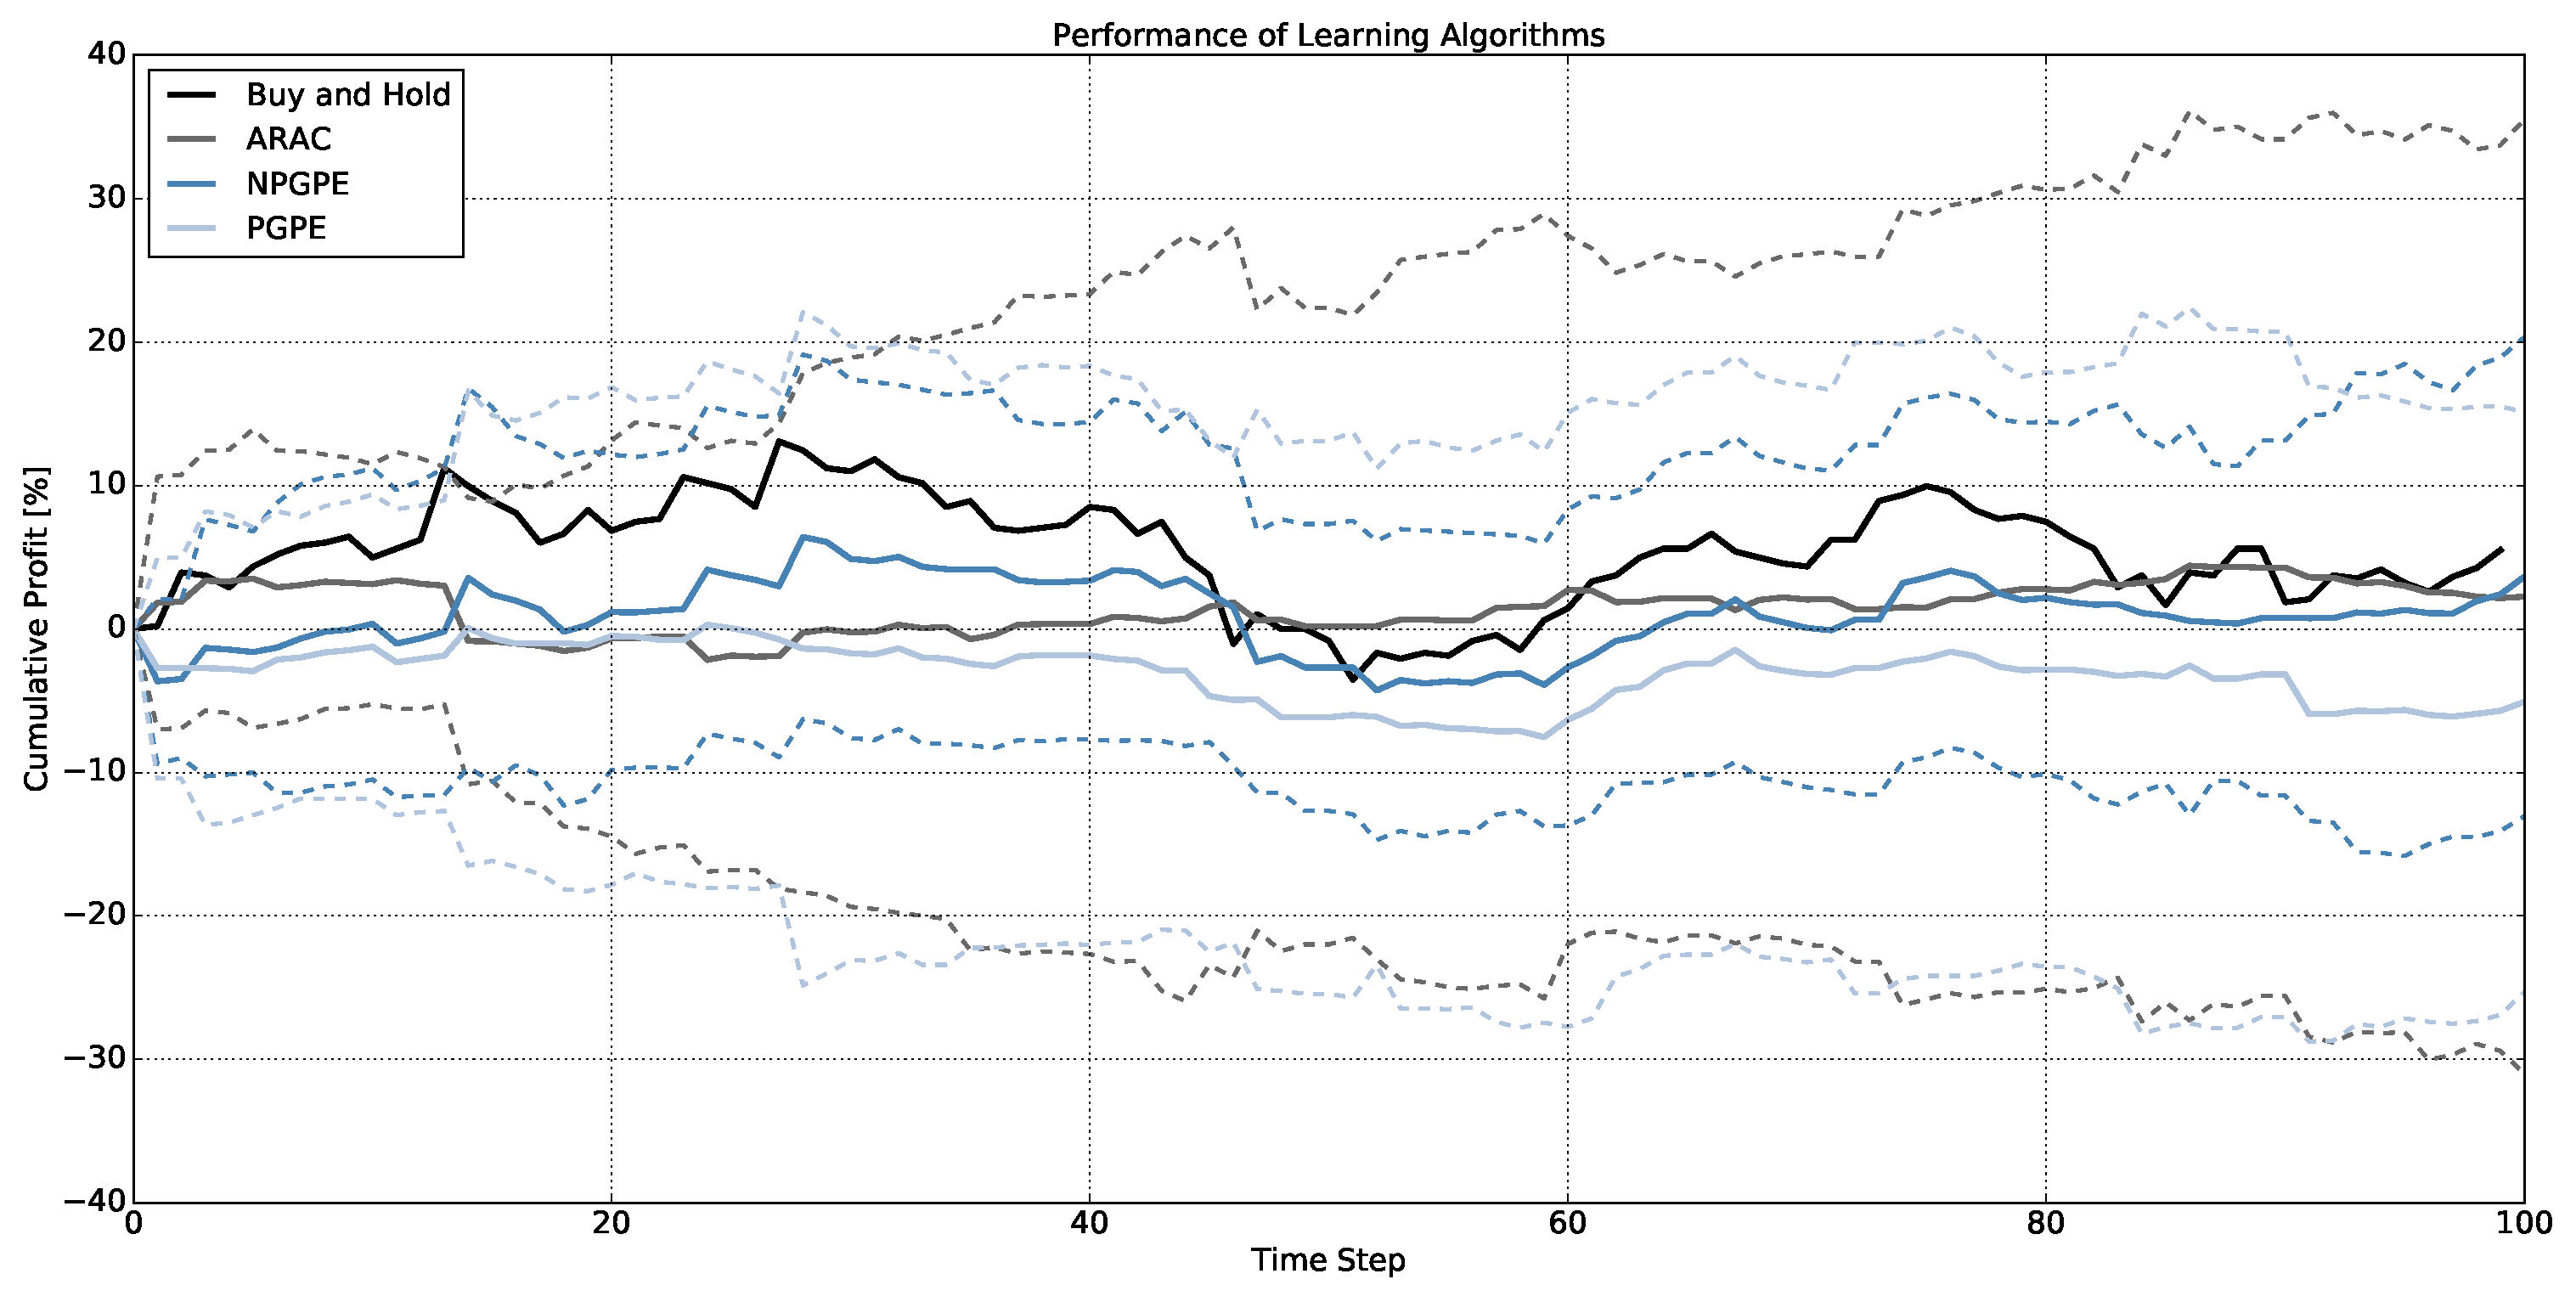
\includegraphics[width=1\textwidth]{Images/8_9_single_hist_neutral_performance}
	     \end{center}
	\end{column}
	\end{columns}
	}
	
	\onslide<2->{	
	\begin{block}{Possible Explanations}
		\begin{enumerate}
			\item<2-> \textbf{Low signal-to-noise ratio}: extremely difficult to find tradable patterns in markets
			\item<3-> \textbf{Quality of data}: unlikely to find patterns in daily prices of liquid stocks
			\item<4-> \textbf{Weak features}: parametric policy must be powerful enough to capture the signal
			\item<5-> \textbf{Non-stationarity of financial time-series}: a signal needs to be persistent
		\end{enumerate}
	\end{block}
	}

\end{frame}

